\section{The Support Vector Machine (SVM)}

\mode<presentation>{
\begin{frame} 
    \begin{center} \huge
        \secname
    \end{center}
    \begin{center}
     Finding the separating hyperplane with maximum margin\\+ the ``kernel trick''   
    \end{center}
\end{frame}
}

\subsection{SVMs are Maximum Margin Classifiers}

\begin{frame}\frametitle{The binary classification setting}

\mode<article>{
The binary classification setting:\\

\begin{figure}[h]
    \centering
    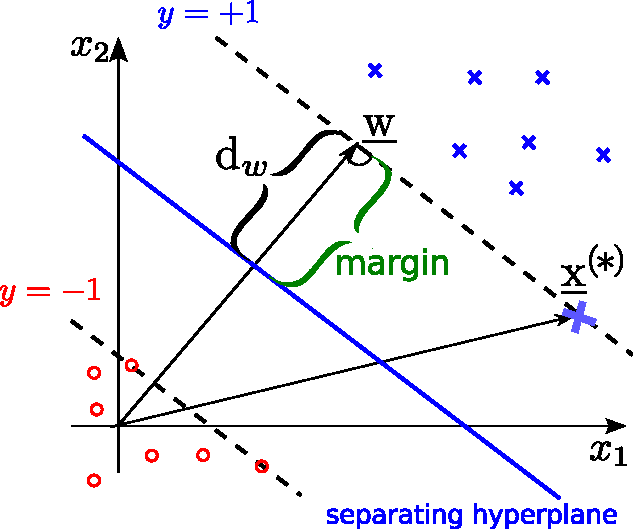
\includegraphics[height=4cm]{img/section2_fig13_v2_space} 
    \mode<article>{
    \caption{
    Binary classification setting.
    }
    \label{fig:setting}
    } 
\end{figure}
}
\mode<presentation>{
\placeimage{8.7}{2.2}{img/section2_fig13_v2_space}{width=4.8cm}
}


\begin{itemize}
	\item \underline{Data}:\\[2mm]
	$
	\Big\{ \left(\vec x^{(\alpha)}, y^{(\alpha)}_{T} \right) \Big\}_{\alpha=1}^{p}\,
	$\\[2mm]
	where $\vec x \in \R^{N}$, $y_T \in \{-1, 1\}$\\

	\item \underline{Model}:\\[2mm]
	$
	y(\vec x; \vec w,b) = \sign \big( \vec w^{\top} \vec x + b \big)
	$
    
    \item \underline{Objective}:
    
    Choose the decision boundary s.t. the margin is \emph{maximal}.
    
    \item \underline{Assumption}:
    
    Perfect linear separation of both classes.
    
    \pause
    
    In the case of a simple connectionist neuron:
    \begin{equation}
    \vec w^{\top} \vec x + b \;\;
    \left \{ \begin{array}{ll}
					\ge& 0 \;\;\text{for } {\color{blue}y_{T} = +1}\\
					<& 0 \;\;\text{for } {\color{red}y_{T} = -1}
				\end{array} \right.  
    \end{equation}
    The solution is not unique.
    
\end{itemize}
    
\end{frame}

\begin{frame}\frametitle{\subsecname}
    \mode<presentation>{
\placeimage{8.7}{2.5}{img/section2_fig13_v2_space}{width=5.5cm}
}
\begin{minipage}{6cm}
Let $\vec w^{*}$ and $b^{*}$ describe the optimal hyperplane that maximizes the margin of separation:
    \begin{equation}
    \vec w^{*\top} \vec x + b^{*} \;\;
    \left \{ \begin{array}{ll}
					\ge& 1 \;\;\text{for } {\color{blue}y_{T} = +1}\\
					\le& -1 \;\;\text{for } {\color{red}y_{T} = -1}
				\end{array} \right.  
    \end{equation}
    
    Points that lie on the margin are characterized by:
    
    \begin{equation}
    \vec w^{*\top} \vec x + b^{*} \;\;
    \left \{ \begin{array}{ll}
					=& 1 \;\;\text{for } {\color{blue}y_{T} = +1}\\
					=& -1 \;\;\text{for } {\color{red}y_{T} = -1}
				\end{array} \right.  
    \end{equation}
    
       

\end{minipage}\\

    These points will be referred to as the \emph{support vectors}.
   \notesonly{
    The shortest distance between points with opposite class labels is $2 \mathrm{d}_{w} = \frac{2}{\lVert \vec w^{*} \rVert}_{2}$, i.e. the distance separating the two classes.
    }
    
    Maximizing the margin $\corresponds$ minimizing the Euclidean norm of $\vec w$. The solution to this is unique.

\end{frame}

\begin{frame}\frametitle{The primal problem for structured risk minimization (SRM)}


The cost function\notesonly{ to minimize}:
    
\begin{equation}
\frac{1}{2} \vec w^{\top} \vec w = \frac{1}{2} \lVert \vec w \rVert_{2}^{2} \eqexcl \min    
\end{equation}

\question{Why have we suddenly switched to the squared Euclidean norm and where did the 2 come form?}

\mode<article>{
- Minimizing the square of the norm turns it into a \emph{convex} minimization problem, which simplifies the optimization procedure.
Dividing by 2 is simply for convinience.
}

We want to restrict the space of solutions for $\vec w$ to that which leads to correct classification of the training points:

We therefore constrain solutions such that:

\begin{equation}
 y_{T}^{(\alpha)} \cdot \big( \vec w^{\top} \vec x^{(\alpha)} + b \big) \ge 1 \;\;\forall \alpha{}
 \label{eq:constraint}
\end{equation}

\notesonly{
\eqref{eq:constraint} provides constraints that are linear in $\vec w$. It is sometimes referred to as the \emph{0-1 loss} or \emph{hinge loss}. It is exactly zero whenever a point is correctly classified and 1 whenever it is misclassified.
}

\notesonly{
This gives us the \emph{primal} problem for structured risk minimization (SRM) prooblem. }The SRM principle is about balancing the complexity of a model while minimizing the tranining error to avoid overfitting.
    
\end{frame}

\begin{frame}
Applying the Lagrange method to the primal problem of SRM:

\begin{equation}
f_{0}(\vec w,b) = \frac{1}{2} \lVert \vec w \rVert_{2}^{2} = \frac{1}{2} \vec w^{\top} \vec w \eqexcl \min
\end{equation}
\notesonly{
Manipulating the constraints \eqref{eq:constraint} to obtain an expression in the form $f_{\alpha} \le 0$:
}

A constraint for each data point in the training set:

\pause

\slidesonly{\vspace{-3mm}}

\begin{align}
 y_{T}^{(\alpha)} \cdot \big( \vec w^{\top} \vec x^{(\alpha)} + b \big) \,\ge\, &1\\
 y_{T}^{(\alpha)} \cdot \big( \vec w^{\top} \vec x^{(\alpha)} + b \big) -1 \,{\color{blue}\ge}\, &0\\
 {\color{blue}-}\big\{y_{T}^{(\alpha)} \cdot \big( \vec w^{\top} \vec x^{(\alpha)} + b \big) -1\big\} \,{\color{blue}\le}\, &0
\end{align}

\begin{equation}
f_{\alpha} (\vec w,b) = -\big\{ y_{T}^{(\alpha)} \cdot \big( \vec w^{\top} \vec x^{(\alpha)} + b \big) -1 \big\} \le 0\;,\quad \alpha = 1,\ldots,p    
\end{equation}

The Lagrangian becomes:

\pause

\slidesonly{\vspace{-5mm}}

\begin{align}
L(\vec w, b, \{\lambda_{\alpha}\}) 
\,=&\, f_{0}(\vec w,b) + \sum_{\alpha=1}^{p} \lambda_{\alpha} f_{\alpha}(\vec w,b)\\
\,=&\, \frac{1}{2} \lVert \vec w \rVert_{2}^{2}
- \sum_{\alpha=1}^{p} \lambda_{\alpha} \big\{ y_{T}^{(\alpha)} \cdot \big( \vec w^{\top} \vec x^{(\alpha)} + b \big) -1 \big\}
\label{eq:lagrangianprimal}\slidesonly{,\quad \lambda_{\alpha} \ge 0}
\end{align}

\end{frame}

\begin{frame}

\mode<presentation>{
\begin{equation*}
L(\vec w, b, \{\lambda_{\alpha}\}) = \frac{1}{2} \lVert \vec w \rVert_{2}^{2}
- \sum_{\alpha=1}^{p} \lambda_{\alpha} \big\{ y_{T}^{(\alpha)} \cdot \big( \vec w^{\top} \vec x^{(\alpha)} + b \big) -1 \big\}
,\quad \lambda_{\alpha} \ge 0
\end{equation*}
}

where $\{\lambda_{a} \ge 0\}_{\alpha=1}^{p}$ is the set of Lagrange multipliers. \notesonly{Because of the minus sign in front of the multipliers, t}\slidesonly{\\[5mm]T}he Lagrangian is optimized by
\begin{itemize}
\item[] \emph{minimizing} w.r.t. $\vec w$ and $b$, the \emph{``primal variables''}, and 
\item[] \emph{maximizing} w.r.t. all $\lambda_{\alpha}$, the \emph{``dual variables''}.
\end{itemize}

\slidesonly{\vspace{5mm}}
This implies that a \emph{saddle point} has to be found for the Lagrangian.
\slidesonly{\vspace{5mm}}

Equivalent optimization problems (Kuhn and Tucker theorem):

\begin{equation}
		{\color{blue}\min_{\vec w, b}}\, L{(\vec{w}, b, {\color{darkgreen} \{ \lambda_\alpha^*\}})}
		= L{({\color{blue}\vec{w}^*}, {\color{blue}b^*}, {\color{darkgreen} \{ \lambda_\alpha^*\}})}
		= {\color{darkgreen}\max_{ \lambda_\alpha \geq 0}}\, L{({\color{blue}\vec{w}^*}, {\color{blue}b^*}, \{ \lambda_\alpha \})}
\end{equation}

\end{frame}


\subsection{Karush-Kuhn-Tucker (KKT) conditions}

\begin{frame}\frametitle{\subsecname}

\only<1-5>{
What is happening as we optimize the Lagrangian of the primal problem?

Recall the constrained optimization problem:

\begin{itemize}
\item[] $\min_{\vec w} \frac{1}{2} \lVert \vec w \rVert_{2}^{2}$
\item[] subject to $-\big\{ y_{T}^{(\alpha)} \cdot \big( \vec w^{\top} \vec x^{(\alpha)} + b \big) -1 \big\} \le 0\;,\quad \text{for all } \alpha = 1,\ldots,p$
\end{itemize}

and the corresponding Lagrangian:

\mode<presentation>{
\slidesonly{\vspace{-5mm}}
\begin{equation}
L(\vec w, b, \{\lambda_{\alpha}\}) = \frac{1}{2} \lVert \vec w \rVert_{2}^{2}
- \sum_{\alpha=1}^{p} \lambda_{\alpha} \big\{ y_{T}^{(\alpha)} \cdot \big( \vec w^{\top} \vec x^{(\alpha)} + b \big) -1 \big\}
,\quad \lambda_{\alpha} \ge 0
\label{eq:lagrangianprimal}
\end{equation}
}



\begin{equation}
		{\color{blue}\min_{\vec w, b}}\, L{(\vec{w}, b, {\color{darkgreen} \{ \lambda_\alpha^*\}})}
		= L{({\color{blue}\vec{w}^*}, {\color{blue}b^*}, {\color{darkgreen} \{ \lambda_\alpha^*\}})}
		= {\color{darkgreen}\max_{ \lambda_\alpha \geq 0}}\, L{({\color{blue}\vec{w}^*}, {\color{blue}b^*}, \{ \lambda_\alpha \})}
\end{equation}
}
\begin{itemize}
\only<1>{\item[]}
\only<2>{
\item
Whenever a constraint is \textcolor{orange}{violated}, i.e.
$
-\big\{ y_{T}^{(\alpha)} \cdot \big( \vec w^{\top} \vec x^{(\alpha)} + b \big) -1 \big\} \,{\color{orange}\le}\, 0
$
\notesonly{
Increasing the value of the corresponding multiplier $\lambda_\alpha$ \emph{\textcolor{darkgreen}{increase}} $L$. 
This will in turn lead to a change in the primal variables $\vec w$ and $b$ to \emph{\textcolor{blue}{decrease}} $L$.
}
\slidesonly{
$\lambda_\alpha \uparrow \quad \leadsto\quad L {\color{darkgreen}\uparrow} \quad \leadsto\quad \text{change in } \vec w,b \quad \leadsto\quad L {\color{blue}\downarrow}$\\
}
}
\only<3>{
\item
\emph{\textcolor{blue}{Decrease}} of $L$ by changing $\vec w$ and $b$ prevents terms inside the sum from taking on arbitrarily large negative values.
}
\only<4>{
\item
Constraints that are not exactly met as equalities, i.e. $-\big\{ y_{T}^{(\alpha)} \cdot \big( \vec w^{\top} \vec x^{(\alpha)} + b \big) -1 \big\} {\color{magenta}{<}} 0$, $L$ can only be maximized by setting the corresponding multiplier $\lambda_\alpha$ to zero.
}
\only<5,6>{
\item
Therefore, $\lambda_\alpha \ne 0$ will correspond to the constraints being met with equality, i.e. $-\big\{ y_{T}^{(\alpha)} \cdot \big( \vec w^{\top} \vec x^{(\alpha)} + b \big) -1 \big\} {\color{red}{=}} 0$. 

\question{What does ``${\color{red}{=}} 0$'' imply w.r.t. misclassification?}

\notesonly{
-This implies that the choice of $\vec w$ and $b$ not only leads to correct classification of that training point but also that the point lies exactly on the margin, indicating that the point for which $\lambda_\alpha \ne 0$ is a \emph{support vector} (cf. \figref{fig:setting}). These are referred to as the \emph{Karush-Kuhn-Tucker (KKT) conditions}.
}
}
\only<6>{
\begin{figure}[h]
    \centering
    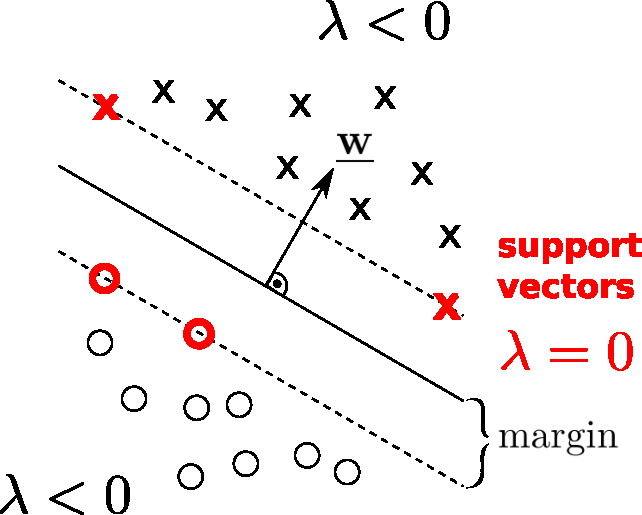
\includegraphics[height=4.5cm]{img/section2_fig18_sv} 
    \mode<article>{
    \caption{
    The constraint for supprt vectors is met with equality.
    }
    \label{fig:conditionsv}
    } 
\end{figure}
}
\end{itemize}

\end{frame}

\subsection{Solving the primal problem}

\begin{frame}\frametitle{\subsecname}

\mode<presentation>{
\begin{equation*}
L(\vec w, b, \{\lambda_{\alpha}\}) = \frac{1}{2} \lVert \vec w \rVert_{2}^{2}
- \sum_{\alpha=1}^{p} \lambda_{\alpha} \big\{ y_{T}^{(\alpha)} \cdot \big( \vec w^{\top} \vec x^{(\alpha)} + b \big) -1 \big\}
,\quad \lambda_{\alpha} \ge 0
\end{equation*}
}

\notesonly{
The Lagrangian of the primal problem is solved by finding the saddle point.} At the saddle point, the derivatives of the Lagrangian $L$ w.r.t to the primal variables goes to zero:

\begin{align}
\only<1,2>{
	\frac{\partial L}{\partial {w}_i} \;\eqexcl&\; 0 \quad \text{for } i=1,\ldots,N\\
	}
\only<2>{ 
	{w}_i - \sum\limits_{\alpha = 1}^p \lambda_\alpha
		y_T^{(\alpha)} \mathrm{x}_i^{(\alpha)} \;\eqexcl&\; 0 \\}
\only<3->{
		\Rightarrow\;\; \vec{w}^* =& \kern-4ex\underbrace{\sum_{\alpha = 1}^p \lambda_\alpha 
		y_T^{(\alpha)} \vec{x}^{(\alpha)}}_{
			\substack{	\text{expansion of the weight vector} \\
					\text{in terms of data points}}}	
					 \label{eq:primalsolution1}
}
\end{align}
\begin{align}
\only<3>{
	\frac{\partial L}{\partial b}
	= -\sum_{\alpha = 1}^p \lambda_\alpha y_T^{(\alpha)} &\eqexcl 0\\
	}
\only<4>{
	\sum_{\alpha = 1}^p \lambda_\alpha y_T^{(\alpha)} &\eqexcl 0
 \label{eq:primalsolution2}
	}
\end{align}

\only<4>{
The solution is unique for $\vec w$ but not for the set of multipliers $\{\lambda_{a}\}_{\alpha=1}^{p}$ (\notesonly{we haven't forgotten about $b^{*}$, }we will get to $b^{*}$ shortly).
}

\end{frame}

\subsection{From the primal problem to the dual problem}

\begin{frame}\frametitle{\subsecname}

\mode<presentation>{
\slidesonly{\vspace{-5mm}}
\begin{equation}
L(\vec w, b, \{\lambda_{\alpha}\}) = \frac{1}{2} \lVert \vec w \rVert_{2}^{2}
- \sum_{\alpha=1}^{p} \lambda_{\alpha} \big\{ y_{T}^{(\alpha)} \cdot \big( \vec w^{\top} \vec x^{(\alpha)} + b \big) -1 \big\}
,\quad \lambda_{\alpha} \ge 0
\label{eq:lagrangianprimal}
\end{equation}
}
    
The \emph{dual} problem: Solving the primal problem \slidesonly{(above)} in addition to finding a unique solution for the set of multipliers.

\pause 

\mode<presentation>{
Solution of the \emph{primal} problem:
\begin{equation}
 \vec w^{*} = \sum_{\alpha=1}^{p} \lambda_{\alpha} y_{T}^{(\alpha)} \vec x^{(\alpha)}
					 \label{eq:primalsolution1}
 \end{equation}

and the condition
\slidesonly{\vspace{-3mm}}
\begin{equation}
 \sum_{\alpha=1}^{p} \lambda_{\alpha} y_{T}^{(\alpha)} = 0 
 \label{eq:primalsolution2} 
\end{equation}
}

\eqref{eq:primalsolution1} and \eqref{eq:primalsolution2} are plugged back into the Lagrangian of the primal problem \eqref{eq:lagrangianprimal}.
\notesonly{From this follows:}

\end{frame}

\begin{frame}\frametitle{From the \emph{primal} problem to the \emph{dual} problem}

\mode<presentation>{
\vspace{-5mm}
\begin{equation}
 \vec w^{*} = \sum_{\alpha=1}^{p} \lambda_{\alpha} y_{T}^{(\alpha)} \vec x^{(\alpha)}
					 \label{eq:primalsolution1}
 \end{equation}
\vspace{-3mm}
\only<1-3>{
\begin{equation}
 \sum_{\alpha=1}^{p} \lambda_{\alpha} y_{T}^{(\alpha)} = 0 
 \label{eq:primalsolution2} 
\end{equation}

\vspace{-2mm}
}
}

\begin{align}
\only<1->{
L(\vec w^*, b, \only<1-3>{&}\{\lambda_{\alpha}\}) \only<1-3>{=\\}
}
\only<1-3>{
=& \frac{1}{2} \vec w^{*\top} \vec w^{*}
- \sum_{\alpha=1}^{p} \lambda_{\alpha} \big\{ y_{T}^{(\alpha)} \cdot \big( \vec w^{*\top} \vec x^{(\alpha)} + b \big) -1 \big\}\\
}
\only<2,3>{
=& \frac{1}{2} \vec w^{*\top} \vec w^{*}
-  \sum_{\alpha=1}^{p} \lambda_{\alpha} y_{T}^{(\alpha)} {\color{blue}\vec w^{*\top}} \vec x^{(\alpha)}
-  \sum_{\alpha=1}^{p} \lambda_{\alpha} y_{T}^{(\alpha)} {\color{blue}b}
+ \sum_{\alpha=1}^{p} \lambda_{\alpha}\\
}
\only<3>{
=& \frac{1}{2} \vec w^{*\top} \vec w^{*}
- {\color{blue}\vec w^{*\top}} \underbrace{\sum_{\alpha=1}^{p} \lambda_{\alpha} y_{T}^{(\alpha)} \vec x^{(\alpha)}}_{= \vec w^* \text{ (cf. \eqref{eq:primalsolution1})}}
- {\color{blue}b} \underbrace{\sum_{\alpha=1}^{p} \lambda_{\alpha} y_{T}^{(\alpha)}}_{= 0 \text{ (cf. \eqref{eq:primalsolution2})}}
+ \sum_{\alpha=1}^{p} \lambda_{\alpha}\\
}
\only<4->{
=& \frac{1}{2} \vec w^{*\top} \vec w^{*}
- {\vec w^{*\top}} \vec w^{*\top}
+ \sum_{\alpha=1}^{p} \lambda_{\alpha}\\
=& -\frac{1}{2} \vec w^{*\top} \vec w^{*}
+ \sum_{\alpha=1}^{p} \lambda_{\alpha}
}
\only<5->{
\intertext{plugging in the solution \notesonly{\eqref{eq:primalsolution1} }for $\vec w^*$:} 
=& -\frac{1}{2} \sum_{\alpha=1}^{p} \lambda_{\alpha} y_{T}^{(\alpha)} {\vec x^{(\alpha)}}^\top \sum_{\beta=1}^{p} \lambda_{\beta} y_{T}^{(\beta)} \vec x^{(\beta)}
+ \sum_{\alpha=1}^{p} \lambda_{\alpha}\\
=& -\frac{1}{2} 
\sum_{\alpha=1}^{p} \sum_{\beta=1}^{p} 
\lambda_{\alpha} \lambda_{\beta} 
y_{T}^{(\alpha)} y_{T}^{(\beta)}
{\vec x^{(\alpha)}}^\top  \vec x^{(\beta)}
+ \sum_{\alpha=1}^{p} \lambda_{\alpha}
} \eqexcl \max_{\{\lambda_\alpha\}}
\label{eq:lagrangiandual}
\end{align}

\mode<article>{
\eqref{eq:lagrangiandual} gives us the maximization objective of the \emph{dual problem}.
}
\end{frame}

\subsection{The dual problem}

\begin{frame}\frametitle{\subsecname}

Find the Lagrange multipliers $\{\lambda_{\alpha}\}$ that maximize:

\mode<presentation>{


\begin{equation}
L(\vec w^*, b, \{\lambda_{\alpha}\})
= -\frac{1}{2} 
\sum_{\alpha=1}^{p} \sum_{\beta=1}^{p} 
\lambda_{\alpha} \lambda_{\beta} 
y_{T}^{(\alpha)} y_{T}^{(\beta)}
{\vec x^{(\alpha)}}^\top  \vec x^{(\beta)}
+ \sum_{\alpha=1}^{p} \lambda_{\alpha}
 \eqexcl \max_{\{\lambda_\alpha\}}
\label{eq:lagrangiandual}
\end{equation}

subject to 
\begin{itemize}
\item[] $\lambda_\alpha \ge 0,\;\; \alpha = 1,\ldots,p$ and
\item[]$\sum_{\alpha=1}^{p} \lambda_{\alpha} y_{T}^{(\alpha)} = 0$
\end{itemize}

Reuse the solution of the primal problem for $\vec w^*$:
\vspace{-5mm}
\begin{equation}
 \vec w^{*} = \sum_{\alpha=1}^{p} \lambda_{\alpha} y_{T}^{(\alpha)} \vec x^{(\alpha)}
					 \label{eq:primalsolution1}
 \end{equation}
 }

This is optimized numerically using \emph{Sequential Minimal Optimization}


\end{frame}

\begin{frame}
Finding $b^{*}$    
\end{frame}

\begin{frame}

\question{What about non-linearly separable classes?}

kernel trick
    
\end{frame}

\subsection{C-SVM}

\begin{frame}

\question{What if the two classes are still not perfectly separable?}

- C-SVMs

No longer assume a perfect separation between the classes:

    
\end{frame}
